\chapter{Design of Mars} \label{sec-design}

In this chapter, we present our design for Mars, with emphasis on the GPU-based component.
Our design is guided by the following three goals.

\begin{enumerate}
  \item {\em Programmability}. User code size reduction encourages programmers to use the GPU for their tasks.
  \item {\em Flexibility}. The design should be applicable to various multi-/many-core processors, e.g., multi-core CPUs and AMD GPUs, and should be as expressive as the underlying runtime, e.g., NVIDIA CUDA, AMD Brook+ or pthreads, so that the system will work for a wide range of hardware and applications.
  \item {\em High Performance}. The overall performance should be accelerated by the GPU effectively.
\end{enumerate}

\section{Overview}
\red{By examining the Phoenix design, we see that there are three potential sources of overhead.  First, the tight-coupling of the Map and Reduce stages makes every application go through both stages, no matter whether they need both stages or not. Second, a dynamic thread scheduler for task assignment heavily relies on locking to implement synchronization. Third, each reduce worker may require frequent data movement for sorting the static output array, and the data movement can become a bottleneck for the overall performance. The latest paper about Phoenix also points out this problem~\cite{Yoo2009}.}


In the Mars design, we decide to separate a MapReduce workflow into three loosely coupled stages -
{\em Map}, {\em Group} and {\em Reduce}. The {\em Group} stage is designed to group {\em Map} output by key, which is the format for {\em Reduce} input. Our observation is that some applications need only the
{\em Map} stage, some need both {\em Map} and {\em Group}, and some need all of the three stages.
\red{The Group stage is the same as running Reduce with the identity function in the original MapReduce system \cite{Dean2008}.
Our purpose of providing an explicit Group stage is to allow a MapReduce application with high flexibility to customize its workflow,
and to avoid the overhead of entering unnecessary stages. }
No matter what configuration of the three stages is for an application, the MapReduce interface
of Mars is unchanged - users write Map and/or Reduce functions when necessary.

Moreover, we decide to use a lock-free scheme for synchronization
and to perform in-advance buffer allocation. One reason is to
avoid heavy overheads of locking and buffer reallocation. The
other reason is that, current GPUs do not support locking
or in-flight buffer reallocation. In our design, we statically
distributes tasks to a massive number of GPU threads, so that we
can fully utilize the parallelism of the GPU. We adopt a two-phase,
lock-free scheme for result output. The basic idea is that, in the
first phase, we calculate histograms on the size of output results for each
thread, followed by a prefix sum operation on the histograms,
so that we obtain both the exact output buffer size and the deterministic
write position for each thread; in the second phase, we
perform the actual computation and output. We will detail this strategy in
Section~\ref{sec-lockfree}.

\section{Data Structure} \label{sec-datastructure}
Data structures in Mars affect the workflow, memory access patterns, and the expressiveness of the system.

Since the GPU does not support dynamic memory allocation on the
device memory during the execution of the GPU code, this limitation rules out
 dynamic data structures such as queues and linked lists, as used in
other MapReduce implementations. Instead, we use plain arrays as the
main data structure in Mars. The {\em Map} stage takes input records in
the key/value form, and outputs intermediate result records, which
are in turn the input of the {\em Group} stage. The output of the {\em Group}
stage is the input of the {\em Reduce} stage, and {\em Reduce} produces final output
records. Each of the three sets - the input records, the intermediate records and the
output records  - is stored in three arrays, i.e., the
key array, the value array and the directory index array. The
directory index consists of an entry of $<$key offset, key size,
value offset, value size$>$ for each key/value pair. Given a
directory index entry, we fetch the key or the value at the
corresponding offset in the key array or the value array.

Variable-sized types, such as strings, are supported with the directory index, since current GPUs have no such build-in types yet. If
two key/value pairs need to be swapped, we swap their corresponding
entries in the directory index without modifying the key and the
value arrays.

Some applications perform chained MapReduce procedures,
where the output of one MapReduce procedure is the input of
another one. Since the sets of
input records, intermediate records and output records  are all
in the three-array structure uniformly, chained MapReduce is
supported gracefully in Mars.

\section{Mars Workflow}
Figure \ref{fig:MarsWorkflow} illustrates the workflow of Mars, assuming the data resides in the disk at the beginning.
The Mars scheduler runs on the CPU, and schedules tasks to the GPU.
Mars has three stages, {\em Map}, {\em Group}, and {\em Reduce}.

\begin{figure}[ht]
  \centering
  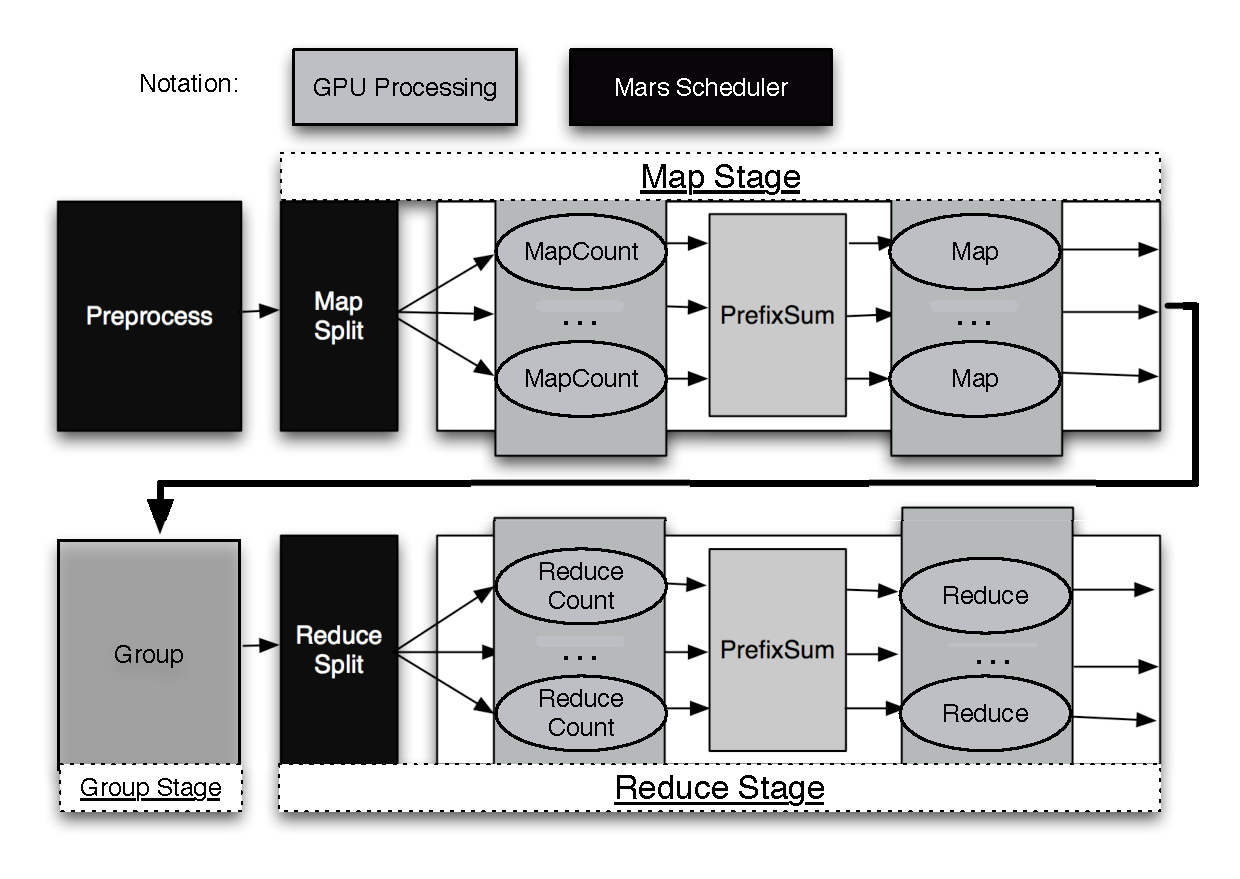
\includegraphics[width=0.60\textwidth]{figure/Mars_workflow.eps}
  \caption{The workflow of Mars on the GPU. }\label{fig:MarsWorkflow}
\end{figure}

Before the {\em Map} stage, Mars preprocesses on the CPU the input data from disk,
transforming the input data to key/value pairs (input records) in main memory.
After that, it transfers input records from the main memory to the GPU device memory.

In the {\em Map} stage, {\em Map Split} dispatches
input records to GPU threads such that the workload for all threads is even.
Each thread executes the user-defined MapCount function to compute a local histogram on
the number and the total size of intermediate records that {\em Map} will output.
Then, the runtime performs a GPU-based {\em Prefix Sum} on the local histograms to
obtain the output size and the write position for each thread.
Finally, after the CPU allocates the output buffer in the device memory, each GPU
thread executes the user-defined Map function and outputs results.  Since the write
position for each thread is pre-computed and has no conflict with any other threads,
there will be no write conflict between concurrent threads. This lock-free scheme of MapCount,
Prefix Sum, and Map is adapted from our previous
work~\cite{He2008a}.

\red{In the {\em Group} stage, both sort-based and hash-based approaches are available for grouping records by key. However, we adopt the sort-based, because some applications require to sort all output records, and the hash-based approach has to perform additional sort within each hash bucket. }


In the {\em Reduce} stage, {\em Reduce Split} dispatches each group of records
with the same key to a GPU thread.
However, it may cause load imbalance between threads, since the number of records of different groups may vary widely.
We adopt a skew handling scheme to alleviate the load imbalance problem (Section~\ref{sec-reduce}).
The {\em Reduce} stage then works in a lock-free scheme, similar to that in {\em Map}, to obtain the result size and the write location for each thread.
Finally, all Reduce workers output results to a single buffer.

Because these three stages are loosely coupled and not every application requires all
stages, Mars allows users to customize the following workflows in their applications:
\begin{itemize}
\item MAP\_ONLY. Mars executes the {\em Map} stage only, and does not execute the {\em Group} or {\em Reduce} stage.
\item MAP\_GROUP. Mars executes the {\em Map} and {\em Group} stages, and does not execute the {\em Reduce} stage.
\item MAP\_GROUP\_REDUCE.  Mars executes all three stages -- {\em Map}, {\em Group}, and {\em Reduce} stages.
\end{itemize}

Because usually applications need a Map to transform input records, and a Group to
prepare for the intermediate records to feed to Reduce, we exclude the other
workflow configurations that skip either Map or Group in the presence of Reduce.

\section{Lock-free Scheme} \label{sec-lockfree}

With the array structure, we allocate the space on the device memory
for the input data as well as for the result output before executing
the GPU program. However, the sizes of the output from the {\em Map} and
the {\em Reduce} stages are unknown. Moreover, write conflicts occur when
multiple threads write results to the shared output array. To
address these two problems, we adopt a previous lock-free output
scheme for relational joins~\cite{He2008a}. Since the output scheme
for the {\em Map} stage is similar to that for the {\em Reduce} stage, we
present the scheme for the {\em Map} stage only.

First, each MapCount invocation on a thread outputs three counts, i.e.,
the number of intermediate results, the total size of intermediate keys (in bytes)
and the total size of intermediate values (in bytes).
Based on intermediate key sizes (or value sizes),
Mars computes a prefix sum on these sizes and produces an array of write locations.
A write location is the start location in the output array for a map task to write.
Based on the number of intermediate results,
Mars computes a prefix sum and produces an array of start locations in the output
directory index.
Through these prefix sums, we also know the sizes of the arrays for the intermediate
results.
Finally, Mars allocates arrays in the device memory with the exact sizes for
storing the intermediate results.

Second, each Map invocation on a thread outputs the intermediate key/value pairs to
the output array.
Since each Map has its deterministic and non-overlapping positions to write to,
the write conflicts are avoided.


The lock-free scheme is suitable for the massive thread parallelism on the GPU, even
though it performs a MapCount in addition to a Map. The overhead of executing MapCount
is application dependent, and is usually small. For example, this overhead is negligible
in the matrix multiplication in our study, since MapCount simply emits the size without
performing the actual multiplication. In addition, the code for MapCount function is also application dependent, while in most cases, programmers write one statement to emits output data sizes. 

\red{
\section{Rapid Group} \label{sec-rapid}
The Group stage requires to sort intermediate records.
However, we observe that some applications inherently have their intermediate records grouped after the Map phase, and each group has the same number of records.
For example, [A,A,A,B,B,B,C,C,C] shows three groups with A, B, and C as the key respectively, and each group is with the same size 3.
For such applications, Mars provides a configuration parameter for users to indicate whether the intermediate data is already grouped. The runtime automatically skips the time consuming sorting, and then dispatches each group of intermediate records with the same group size to Reduce workers.
We name this strategy as ``Rapid Group".
}

\section{Skew handling} \label{sec-reduce}

We design a skew handling scheme to distribute workloads evenly across reduce workers, where the user-defined Reduce operation is commutative and associative.
This scheme iteratively performs the {\em Reduce} stage in the following two steps.  First, we divide the data into $M$ equal-sized chunks.  Second, we perform a reduction on each chunk. In this step, each of the $M$ threads applies the reduce function on groups of records in a single chunk.  Note, in each iteration, we perform reduction on the intermediate results with the same keys only.

%This scheme starts within the {\em Group} stage, immediately after the sorting, and performs in the following three steps.  First, we divide the data into $M$ equal-sized chunks. Second, we perform a reduction on each chunk.  In this step, each of the $M$ threads applies the reduce function on groups of records in a single chunk, called {\em local reduction}.  Finally, we group the reduced intermediate results and pass them to the {\em Reduce} stage.  This skew handling scheme makes sure that {\em local reduction} in {\em Group} stage are load-balanced.  Additionally, the {\em Reduce} stage processes compact groups of records, so that it alleviates the bottleneck caused by the largest group.

\section{Mars APIs}
Mars provides a small set of APIs. Similar to the existing MapReduce
frameworks, Mars has two kinds of APIs, the user-implemented APIs,
which the users should implement by themselves, and the
system-provided APIs, which the users can use as library calls.
%We refer the readers to our conference paper~\cite{He2008} for more details about Mars APIs.
The definitions of these APIs are in Table \ref{tb:marsapi}.

\doublerulesep 0.1pt
\begin{table}[htb]
  \centering
 \linespread{1.7}{ {\footnotesize
  \caption{Mars APIs}\label{tb:marsapi}
\vspace{2em}
  \begin{tabular}{p{5cm}p{7.5cm}p{3.5cm}}
  \hline
\noalign{\smallskip}
   \textbf{Function Name} & \textbf{Description} & \textbf{Function Type}\\
\noalign{\smallskip}
  \hline
   MAP\_COUNT & It calculates the output buffer size of MAP. & User-implemented \\
   MAP & The map function. & User-implemented \\
   REDUCE\_COUNT & It calculates the output buffer size of REDUCE. & User-implemented \\
   REDUCE & The reduce function. & User-implemented \\
   EMIT\_INTERMEDIATE\_COUNT & It emits the key size and the value size in MAP\_COUNT. & System-provided \\
   EMIT\_INTERMEDIATE & It emits the key and the value in MAP. & System-provided \\
   EMIT\_COUNT & It emits the key size and the value size in REDUCE\_COUNT. & System-provided \\
   EMIT & It emits the key and the value in REDUCE. & System-provided \\
\noalign{\smallskip}
  \hline
  \end{tabular}
  }}
\end{table}



\newpage
